\subsection{RQ3: Can open-source LLM detect SATD in test code?}
\textbf{Motivation.} Although SATD often contains keywords such as \textit{TODO}, many comments do not follow such patterns. In these cases, even sophisticated pattern-based methods (e.g., TM, NLP) fail to detect SATD, highlighting the need for approaches that capture semantic meaning. Consequently, we investigate Large Language Models (LLMs), given their strong capability in understanding both natural language and source code~\cite{brown_language_2020}. Recent studies have also found promising results with LLMs for detecting source code SATD~\cite{sheikhaei_empirical_2024, lambert_identification_2024}, outperforming conventional approaches.
\begin{figure}
    \centering
    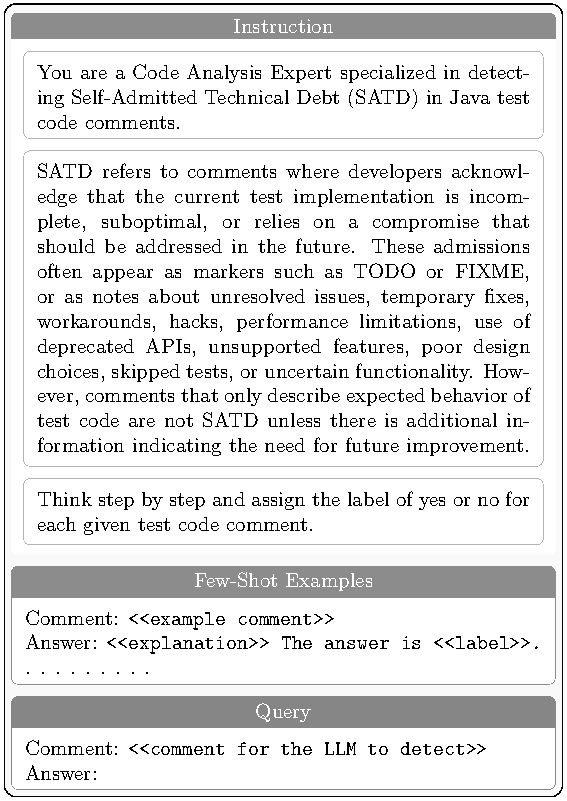
\includegraphics[width=\textwidth,
        height=0.95\textheight,
        keepaspectratio]{figure/satd-detection-prompt-template.pdf}
    \caption{LLM prompt template for detecting SATD comment.}
    \label{fig:satd-detection-prompt-template}
    % \Description{LLMs template for detecting SATD comment with structured UI-style layout.}
\end{figure}

\textbf{Approach.} Encouraged by the success of SATD detection~\cite{sheikhaei_empirical_2024} of the Flan-T5 model series, we investigated these models on test code SATD with few-shot configurations of 0, 2, and 4 shots. These models are T5-SMALL, T5-BASE, T5-LARGE, T5-XL, and T5-XXL, with numbers of parameters 60M to 11B. The experiments were run on an HPC cluster with Intel 8570 CPUs (2.1 GHz) and multiple NVIDIA H100 GPUs. We tested four different prompt templates: No Keyword, MAT, Jitterbug, and GPT-4. These were adopted from Sheikhaei et al.~\cite{sheikhaei_empirical_2024} to enable direct comparison with their results. 

Additionally, we added a new prompt template that we mainly developed for RQ4, as illustrated in Figure~\ref{fig:satd-detection-prompt-template}. Existing research highlights that LLMs are highly sensitive to the structure and phrasing of prompts, with their performance varying considerably depending on how tasks, instructions, and examples are articulated~\cite{liu_pre-train_2023}. To ensure greater reliability and adaptability, a modular prompt template was developed, comprising three components, in accordance with established prompt design frameworks~\cite{amatriain_prompt_2024, giray_prompt_2023}. The first, the Instruction, is organized into three parts: (i) a role-based persona that anchors the model’s behavior and enhances response quality~\cite{hu_quantifying_2024}; (ii) a contextual and task-specific description that clarifies the model’s objective~\cite{amatriain_prompt_2024}; and (iii) explicit output formatting guidelines that reduce ambiguity and improve consistency in responses. The second, Few-Shot Examples, varies in number across experiments to assess performance sensitivity. Finally, the third, Query, contains the target comment that the LLM is required to analyze and classify.


\begin{table*}[ht!]
% \centering
% \caption{Precision (P), Recall (R), F1-score (F1), and Matthews Correlation Coefficient (MCC) for detecting SATD comments using Flan-T5 series open-source LLMs across 0-, 2-, and 4-shot settings. Keyword-based prompts (e.g., MAT, Jitterbug) generally achieve higher F1-scores, whereas smaller models and No Keyword/GPT-4–suggested prompts often fail to identify SATD.}
\caption{Precision (P), Recall (R), F1-score (F1), and Matthews Correlation Coefficient (MCC) for detecting SATD comments using Flan-T5 series open-source LLMs across 0-, 2-, and 4-shot settings.}
\label{table:oss_llm_detection_result}

% \resizebox{\textwidth}{!}{
% \small
% \setlength{\tabcolsep}{3pt}
\renewcommand{\arraystretch}{0.9}
\begin{adjustbox}{max width=\textwidth, max height=\textheight}
\begin{tabular}{ccccccccccccccc}
\toprule
% \multirow{2}{*}{\textbf{Dataset}} & \multirow{2}{*}{\textbf{Prompt}} & \multirow{2}{*}{\textbf{Model}}
% & \multicolumn{4}{c}{\textbf{0-shot}}
% & \multicolumn{4}{c}{\textbf{2-shots}}
% & \multicolumn{4}{c}{\textbf{4-shots}} \\
\multirow{2}{*}{\rotatebox[origin=c]{45}{\textbf{Dataset}}}
& \multirow{2}{*}{\rotatebox[origin=c]{45}{\textbf{Prompt}}}
& \multirow{2}{*}{\textbf{Model}}
& \multicolumn{4}{c}{\textbf{0-shot}}
& \multicolumn{4}{c}{\textbf{2-shots}}
& \multicolumn{4}{c}{\textbf{4-shots}} \\
\cmidrule(lr){4-7} \cmidrule(lr){8-11} \cmidrule(lr){12-15}
 &  &  & \textbf{P} & \textbf{R} & \textbf{F1} & \textbf{MCC}
 & \textbf{P} & \textbf{R} & \textbf{F1} & \textbf{MCC}
 & \textbf{P} & \textbf{R} & \textbf{F1} & \textbf{MCC} \\[0.8em]
\midrule
\multirow{25}{*}{\rotatebox[origin=c]{90}{Original}}&\multirow{5}{*}{\centering New} & T5-SMALL  & 0.00 & 0.02 & 0.01 & -0.02  & 0.00 & 0.00 & 0.00 & -0.01  & 0.00 & 0.00 & 0.00 & -0.01  \\
& & T5-BASE  & 0.01 & 0.31 & 0.02 & -0.03  & 0.02 & 0.51 & 0.03 & 0.01  & 0.01 & 0.45 & 0.03 & 0.01  \\
& & T5-LARGE  & 0.03 & 0.96 & 0.05 & 0.10  & 0.04 & 0.91 & 0.07 & 0.14  & 0.04 & 0.74 & 0.07 & 0.12  \\
& & T5-XL  & 0.29 & 0.86 & 0.43 & 0.49  & 0.38 & 0.79 & 0.51 & 0.54  & 0.47 & 0.64 & 0.54 & 0.54  \\
& & T5-XXL  & 0.10 & \textbf{0.98} & 0.18 & 0.29  & 0.12 & 0.96 & 0.21 & 0.32  & 0.11 & 0.95 & 0.20 & 0.31  \\
\cmidrule(lr){2-15}
&\multirow{5}{*}{\centering \makecell{No\\Keyword}} & T5-SMALL  & 0.00 & 0.00 & 0.00 & 0.00  & 0.00 & 0.00 & 0.00 & 0.00  & 0.00 & 0.00 & 0.00 & 0.00  \\
& & T5-BASE  & 0.00 & 0.03 & 0.01 & -0.04  & 0.00 & 0.00 & 0.00 & 0.00  & 0.00 & 0.00 & 0.00 & -0.00  \\
& & T5-LARGE  & 0.00 & 0.00 & 0.00 & 0.00  & 0.00 & 0.00 & 0.00 & 0.00  & 0.00 & 0.00 & 0.00 & 0.00  \\
& & T5-XL  & 0.33 & 0.01 & 0.01 & 0.05  & 0.00 & 0.00 & 0.00 & 0.00  & 0.00 & 0.00 & 0.00 & 0.00  \\
& & T5-XXL  & 0.10 & 0.66 & 0.18 & 0.24  & 0.19 & 0.50 & 0.28 & 0.29  & 0.17 & 0.50 & 0.25 & 0.28  \\
\cmidrule(lr){2-15}
&\multirow{5}{*}{\centering GPT 4} & T5-SMALL  & 0.00 & 0.00 & 0.00 & 0.00  & 0.00 & 0.00 & 0.00 & 0.00  & 0.00 & 0.00 & 0.00 & 0.00  \\
& & T5-BASE  & 0.01 & 0.04 & 0.01 & -0.03  & 0.00 & 0.00 & 0.00 & -0.00  & 0.00 & 0.00 & 0.00 & -0.02  \\
& & T5-LARGE  & 0.24 & 0.04 & 0.06 & 0.09  & 0.29 & 0.01 & 0.03 & 0.06  & 0.67 & 0.01 & 0.03 & 0.10  \\
& & T5-XL  & \textbf{1.00} & 0.04 & 0.07 & 0.19  & 0.00 & 0.00 & 0.00 & 0.00  & 0.00 & 0.00 & 0.00 & 0.00  \\
& & T5-XXL  & 0.20 & 0.87 & 0.32 & 0.40  & 0.18 & 0.82 & 0.30 & 0.37  & 0.18 & 0.80 & 0.30 & 0.36  \\
\cmidrule(lr){2-15}
&\multirow{5}{*}{\centering Jitterbug} & T5-SMALL  & 0.00 & 0.00 & 0.00 & 0.00  & 0.00 & 0.00 & 0.00 & 0.00  & 0.00 & 0.00 & 0.00 & 0.00  \\
& & T5-BASE  & 0.00 & 0.03 & 0.01 & -0.03  & 0.00 & 0.00 & 0.00 & -0.00  & 0.00 & 0.00 & 0.00 & -0.01  \\
& & T5-LARGE  & 0.00 & 0.00 & 0.00 & 0.00  & 0.00 & 0.00 & 0.00 & 0.00  & 0.00 & 0.00 & 0.00 & 0.00  \\
& & T5-XL  & \textbf{1.00} & 0.47 & 0.64 & 0.68  & \textbf{1.00} & 0.11 & 0.20 & 0.33  & \textbf{1.00} & 0.08 & 0.15 & 0.28  \\
& & T5-XXL  & 0.28 & 0.83 & 0.42 & 0.47  & 0.27 & 0.82 & 0.41 & 0.46  & 0.30 & 0.80 & 0.43 & 0.48  \\
\cmidrule(lr){2-15}
&\multirow{5}{*}{\centering MAT} & T5-SMALL  & 0.00 & 0.00 & 0.00 & 0.00  & 0.00 & 0.00 & 0.00 & 0.00  & 0.00 & 0.00 & 0.00 & 0.00  \\
& & T5-BASE  & 0.00 & 0.04 & 0.01 & -0.03  & 0.00 & 0.00 & 0.00 & -0.00  & 0.00 & 0.00 & 0.00 & -0.00  \\
& & T5-LARGE  & 0.00 & 0.00 & 0.00 & 0.00  & 0.00 & 0.00 & 0.00 & 0.00  & 0.00 & 0.00 & 0.00 & 0.00  \\
& & T5-XL  & 0.99 & 0.52 & \textbf{0.68} & \textbf{0.71}  & \textbf{1.00} & 0.13 & 0.23 & 0.36  & \textbf{1.00} & 0.12 & 0.21 & 0.34  \\
& & T5-XXL  & 0.33 & 0.80 & 0.47 & 0.50  & 0.40 & 0.78 & 0.53 & 0.55  & 0.42 & 0.74 & 0.54 & 0.55  \\
\midrule
\multirow{25}{*}{\rotatebox[origin=c]{90}{Deduplicate}}&\multirow{5}{*}{\centering New} & T5-SMALL  & 0.01 & 0.03 & 0.01 & -0.02  & 0.00 & 0.00 & 0.00 & -0.01  & 0.00 & 0.00 & 0.00 & -0.01  \\
& & T5-BASE  & 0.02 & 0.36 & 0.04 & 0.01  & 0.02 & 0.55 & 0.04 & 0.03  & 0.02 & 0.52 & 0.04 & 0.03  \\
& & T5-LARGE  & 0.03 & 0.95 & 0.05 & 0.09  & 0.04 & 0.89 & 0.08 & 0.14  & 0.05 & 0.76 & 0.09 & 0.14  \\
& & T5-XL  & 0.26 & 0.85 & 0.40 & 0.46  & 0.36 & 0.76 & 0.49 & 0.51  & 0.46 & 0.65 & 0.54 & 0.53  \\
& & T5-XXL  & 0.10 & \textbf{0.97} & 0.18 & 0.28  & 0.11 & \textbf{0.97} & 0.20 & 0.31  & 0.11 & 0.96 & 0.20 & 0.30  \\
\cmidrule(lr){2-15}
&\multirow{5}{*}{\centering \makecell{No\\Keyword}} & T5-SMALL  & 0.00 & 0.00 & 0.00 & 0.00  & 0.00 & 0.00 & 0.00 & 0.00  & 0.00 & 0.00 & 0.00 & 0.00  \\
& & T5-BASE  & 0.01 & 0.04 & 0.02 & -0.01  & 0.00 & 0.00 & 0.00 & 0.00  & 0.00 & 0.00 & 0.00 & -0.00  \\
& & T5-LARGE  & 0.00 & 0.00 & 0.00 & 0.00  & 0.00 & 0.00 & 0.00 & 0.00  & 0.00 & 0.00 & 0.00 & 0.00  \\
& & T5-XL  & 0.00 & 0.00 & 0.00 & -0.00  & 0.00 & 0.00 & 0.00 & 0.00  & 0.00 & 0.00 & 0.00 & 0.00  \\
& & T5-XXL  & 0.11 & 0.74 & 0.20 & 0.26  & 0.22 & 0.58 & 0.32 & 0.34  & 0.21 & 0.57 & 0.31 & 0.33  \\
\cmidrule(lr){2-15}
&\multirow{5}{*}{\centering GPT 4} & T5-SMALL  & 0.00 & 0.00 & 0.00 & 0.00  & 0.00 & 0.00 & 0.00 & 0.00  & 0.00 & 0.00 & 0.00 & 0.00  \\
& & T5-BASE  & 0.01 & 0.04 & 0.02 & -0.01  & 0.00 & 0.00 & 0.00 & -0.00  & 0.00 & 0.00 & 0.00 & -0.01  \\
& & T5-LARGE  & 0.25 & 0.04 & 0.07 & 0.10  & 0.29 & 0.02 & 0.03 & 0.07  & 0.67 & 0.02 & 0.03 & 0.11  \\
& & T5-XL  & \textbf{1.00} & 0.04 & 0.07 & 0.19  & 0.00 & 0.00 & 0.00 & 0.00  & 0.00 & 0.00 & 0.00 & 0.00  \\
& & T5-XXL  & 0.19 & 0.87 & 0.31 & 0.39  & 0.18 & 0.87 & 0.29 & 0.37  & 0.18 & 0.83 & 0.30 & 0.37  \\
\cmidrule(lr){2-15}
&\multirow{5}{*}{\centering Jitterbug} & T5-SMALL  & 0.00 & 0.00 & 0.00 & 0.00  & 0.00 & 0.00 & 0.00 & 0.00  & 0.00 & 0.00 & 0.00 & 0.00  \\
& & T5-BASE  & 0.01 & 0.02 & 0.01 & -0.01  & 0.00 & 0.00 & 0.00 & -0.00  & 0.00 & 0.00 & 0.00 & -0.01  \\
& & T5-LARGE  & 0.00 & 0.00 & 0.00 & 0.00  & 0.00 & 0.00 & 0.00 & 0.00  & 0.00 & 0.00 & 0.00 & 0.00  \\
& & T5-XL  & \textbf{1.00} & 0.40 & 0.57 & 0.63  & \textbf{1.00} & 0.12 & 0.22 & 0.35  & \textbf{1.00} & 0.09 & 0.16 & 0.29  \\
& & T5-XXL  & 0.28 & 0.82 & 0.42 & 0.47  & 0.26 & 0.81 & 0.39 & 0.44  & 0.28 & 0.79 & 0.41 & 0.45  \\
\cmidrule(lr){2-15}
&\multirow{5}{*}{\centering MAT} & T5-SMALL  & 0.00 & 0.00 & 0.00 & 0.00  & 0.00 & 0.00 & 0.00 & 0.00  & 0.00 & 0.00 & 0.00 & 0.00  \\
& & T5-BASE  & 0.01 & 0.03 & 0.01 & -0.01  & 0.00 & 0.00 & 0.00 & -0.00  & 0.00 & 0.00 & 0.00 & -0.00  \\
& & T5-LARGE  & 0.00 & 0.00 & 0.00 & 0.00  & 0.00 & 0.00 & 0.00 & 0.00  & 0.00 & 0.00 & 0.00 & 0.00  \\
& & T5-XL  & \textbf{1.00} & 0.46 & \textbf{0.63} & \textbf{0.68}  & \textbf{1.00} & 0.15 & 0.26 & 0.39  & \textbf{1.00} & 0.13 & 0.23 & 0.36  \\
& & T5-XXL  & 0.34 & 0.79 & 0.47 & 0.50  & 0.40 & 0.76 & 0.52 & 0.54  & 0.40 & 0.72 & 0.52 & 0.53  \\
\bottomrule


\end{tabular}%
% }
\end{adjustbox}
\end{table*}


\textbf{Results.} Table~\ref{table:oss_llm_detection_result} reports the results for the T5 model family, ranging from T5-SMALL to T5-XXL. The findings indicate that the Flan-T5 series LLMs are unable to consistently detect SATD in test code, with their effectiveness varying depending on the prompting strategy, shots, and model size. In most cases, the smaller models---T5-Small, T5-Base, and T5-Large---failed to detect SATD, resulting in zero recall and, consequently, zero precision.

Between the two largest models, T5-XL consistently achieved higher precision than T5-XXL, often reaching near-perfect precision (e.g., 1.0) with keyword-based prompts (MAT and Jitterbug). However, this high precision generally came at the expense of very low recall. The Ours prompt performed competitively, achieving a maximum F1-score of 0.54. In contrast, the No Keyword and GPT-4 prompts yielded poor results, with many zero-shot and few-shot runs failing to detect any SATD (F1 = 0.0). Meanwhile, the T5-XXL models demonstrated higher recall, frequently exceeding 0.8, but with substantially lower precision (ranging from 0.10 to 0.42). 

When comparing the F1-scores of T5-XXL across different prompt variations with those reported by Sheikhaei et al.~\cite{sheikhaei_empirical_2024}, we observe similar overall trends; however, the scores in our evaluation are approximately 30\% lower. Overall, the MAT-based keyword prompts achieved the highest F1-score (0.68). This strong performance is largely due to the high prevalence of MAT-suggested keywords—particularly \textit{TODO}—in SATD comments and their absence in non-SATD comments within our test dataset. For instance, using the MAT approach, the model correctly identified 71 SATD comments out of 137 with the Flan-T5-XL (zero-shot) setup but failed to detect the remaining 66, even when other obvious indicators (e.g., yuck, workaround) were present. A clear example of a missed case is the comment \textit{“// kinda sorta wrong, but for testing’s sake...”}, which expresses technical debt but lacks any MAT-suggested keywords.

These findings indicate that the choice of prompt has a substantial impact on model performance. Increasing the number of shots (0→2→4), however, did not consistently improve results; this trend was also observed by Sheikhaei et al.~\cite{sheikhaei_empirical_2024}. In both studies, the best performance was achieved under zero-shot settings, as demonstrated by T5-XL with MAT-based prompts in our experiments. 
% Increasing the number of shots tended to improve recall (e.g., for T5-XL) but often led to a decrease in precision, resulting in marginal or even negative changes in F1-scores.



\begin{tcolorbox}
\textbf{\underline{RQ3 summary}:} 
The results indicate that open-source LLMs (Flan-T5 series) struggle to reliably detect SATD in test code across different prompt types and shot settings. Although the best F1-score reached 0.68 using the MAT prompt, the overall performance remains inconsistent and relatively poor compared to the existing tools (RQ2), suggesting that these models have a limited ability to understand and generalize SATD patterns in test code.
\end{tcolorbox}
